\documentclass[a4paper,12pt]{article} 



%Добавляет возможность искать и копировать текст
\usepackage{cmap}

%Убирает пробел между названием таблицы/рисунка и самой таблицей/рисунком
\usepackage{caption}
\captionsetup[table]{skip= -0 cm}
\captionsetup[figure]{skip= -0 cm}

%Выравнивание названия таблиц по левому краю
%\usepackage[nooneline]{caption} 
%Размеры отступов 
\usepackage[left=20mm, top=20mm, right=20mm, bottom=20mm, footskip=10mm]{geometry}

%Рисунки
\usepackage{graphicx}
\usepackage{wrapfig} %обтекание элементов
\graphicspath{{graphs}{figures}}  % папки с картинками

%Русский язык в формулах
%\usepackage{mathtext}

%  Русский язык
\usepackage[T2A]{fontenc}			
\usepackage[utf8]{inputenc}			
\usepackage[english,russian]{babel}	

%Готические буквы
\usepackage{amssymb}

%Русский язык в формулах
\usepackage{mathtext}

% Математика
\usepackage{amsmath,amsfonts,amssymb,amsthm,mathtools} 
\usepackage{wasysym}

%Цветные подписи в таблице
\usepackage[table,xcdraw]{xcolor}

\usepackage{fancyhdr} % Колонтитулы
 	\pagestyle{fancy}
 	\renewcommand{\headrulewidth}{0.3mm}  % Толщина линейки, отчеркивающей верхний колонтитул
 	%\lfoot{Нижний левый}
 	%\rfoot{Нижний правый}
 	\rhead{Кафедра квантовой электроники}
 	%\chead{Верхний в центре}
 	\lhead{Оптика лазерных пучков}
 	% \cfoot{Нижний в центре} % По умолчанию здесь номер страницы
 	
\begin{document} 

%Титульник 
\begin{titlepage}
	\begin{center}
		\large 	МИНИСТЕРСТВО ОБРАЗОВАНИЯ И НАУКИ РОССИЙСКОЙ ФЕДЕРАЦИИ\\
				МОСКОВСКИЙ ФИЗИКО-ТЕХНИЧЕСКИЙ ИНСТИТУТ \\
				(НАЦИОНАЛЬНЫЙ ИССЛЕДОВАТЕЛЬСКИЙ УНИВЕРСИТЕТ)\\ 
				ФИЗТЕХ-ШКОЛА ЭЛЕКТРОНИКИ, ФОТОНИКИ \\
				И МОЛЕКУЛЯРНОЙ ФИЗИКИ \\
		
		
		\vspace{4.0 cm}
		\LARGE{Отчет по лабораторной работе} \\ 
		\LARGE \textbf{Оптика лазерных пучков} \\
	\end{center}
	\vspace{3 cm} \large

	%Надо подумать как это нормально написать	
	\begin{flushleft}
		Работу выполнили \hspace{5.5cm}  \underline{\hspace{3cm}} А.И.Белостоцкий \\	
		\hspace{9.8cm}  \underline{\hspace{3cm}} И.Мазуренко \\
		\hspace{9.8cm}  \underline{\hspace{3cm}} Е.Ионидис \\
		\hspace{9.8cm}  \underline{\hspace{3cm}} А.Шарапов \\
		\hspace{9.8cm}  \underline{\hspace{3cm}} П.Яшин \\
		\hspace{9.8cm}  \underline{\hspace{3cm}} Н.Плюскова \\
		\vspace{2cm}
		Работу принял, оценка \hspace{4.3cm} \underline{\hspace{3cm}}
	\end{flushleft}
	
	
	\vfill

	\begin{center}
	Долгопрудный, 2022 г.
	\end{center}
\end{titlepage}           

\tableofcontents

\newpage

\section{Аннотация}
В данной работе изучаются основы теории лазерных резонаторов и методы анализа лазерных пучков. Теоретический материал сопровождается задачами и наглядным физическим экспериментом. 
\section{Теоретические основы}

\subsection{Гауссовы оптические системы}

Рассмотрим произвольную оптическую систему, состоящую из участков неоднородной среды, линз, зеркал, призм и остальных элементов.

Пусть на эту систему падает геометрический луч, который в заданной плоскости $z_1 = const$ характеризуется двумя величинами: расстоянием $x_1$ от оси $Z$ и углом наклона к ней $\alpha_1$. Тогда на выходе оптической системы имеем координаты луча:

\begin{equation}
\begin{split}
    x_2 = F(x_1, \alpha_1),\\
    \alpha_2 = \Phi(x_1, \alpha_1),
\end{split}
\end{equation}

\begin{figure}[h!]
    \center{\includegraphics[width=4.5in]{abcd_model.jpg}}
    \caption{Ход луча в произвольной оптической системе}
    \label{fig:abcd}
\end{figure}

где $F$ и $\Phi$ -- некоторые функции. Разложим данные функции в ряд Тейлора:

\begin{equation}
\begin{split}
    x_2 = Ax_1 + B\alpha_1 + a_1 x_1^2 + a_2 x_1 \alpha_1 + a_3 \alpha_1^2 + \dots,\\
    \alpha_2 = Cx_1 + D\alpha_1 + b_1 x_1^2 + b_2 x_1 \alpha_1 + b_3 \alpha_1^2 + \dots,
\end{split}
\label{dissolve}
\end{equation}

где $A = \frac{\partial F}{\partial x_1}\Bigr|_{\substack{x_1=0\\\alpha_1=0}}$, $B = \frac{\partial F}{\partial \alpha_1}\Bigr|_{\substack{x_1=0\\\alpha_1=0}}$, $C = \frac{\partial \Phi}{\partial x_1}\Bigr|_{\substack{x_1=0\\\alpha_1=0}}$, $D = \frac{\partial \Phi}{\partial \alpha_1}\Bigr|_{\substack{x_1=0\\\alpha_1=0}}$ -- производные первого порядка, $a_i$, $b_i$ -- производные функций $F$ и $\Phi$ второго порядка.

Если в разложении (\ref{dissolve}) можно пренебречь всеми членами, кроме линейных, то оптическая система называется \textit{гауссовой} (ГОС)

Для ГОС имеем:

\begin{equation}
\begin{split}
    x_2 = Ax_1 + B\alpha_1,\\
    \alpha_2 = Cx_1 + D\alpha_1.
\end{split}
\end{equation}

Перепишем соотношения в матричном виде:

\begin{equation}
    \begin{pmatrix}
        x_2\\
        \alpha_2
    \end{pmatrix}
    =
    \begin{pmatrix}
        A & B\\
        C & D
    \end{pmatrix}
    \begin{pmatrix}
        x_1\\
        \alpha_1
    \end{pmatrix}.
\end{equation}

Матрицу коэффициентов A, B, C, D называют \textit{лучевой матрицей} системы.

\subsection{Оптика гауссовых пучков}

Воспользуемся скалярной теорией дифракции, чтобы проанализировать распространение пучков света через ГОС.
В оптике доказывается, что если на ГОС с лучевой матрицей M падает волновой пучок, в котором поперечное распределение какой-либо компоненты вектора поля описывается функцией $U(x_1, y_1)$, то на выходе системы будет пучок с распределением

\begin{multline}
    U_2 (x_2, y_2) = \frac{ie^{-ikl}}{\lambda B} \int\int_{-\infty}^{+\infty}U(x_1,y_1)dx_1 dy\times
    \exp{(-\frac{ik}{2B}[A(x_1^2+y_1^2)+D(x_2^2+y_2^2)-2(x_1 x_2 + y_1 y_2)])},
    \label{equ:prop}
\end{multline}

где $A$, $B$, $D$ -- компоненты лучевой матрицы системы, $l$ -- геометрическая длина системы, $k = 2\pi/\lambda$ -- волновой вектор, а $\lambda$ -- длина волны. Интегрирование ведётся по входной плоскости оптической системы.

Пучок не ограничен апертурой, так как апертура не является гауссовым элементом.

В простейшем случае, когда оптическая система представляет собой участок свободного пространства длиной $l$, $A = D = 1$, $B = l$, и выражение (\ref{equ:prop}) переходит в \textit{формулу Гюйгенса-Френеля}, записанную в параксиальном приближении:

\begin{equation}
    U_2 (x_2, y_2) = \frac{ie^{-ikl}}{\lambda l}\int\int_{-\infty}^{+\infty}U(x_1,y_1)dx_1 dy_1\times
    \exp{(-\frac{ik}{2l}[(x_2 - x_1)^2 + (y_2 - y_1)^2])}.
\end{equation}

При распространении в свободном пространстве поперечная структура пучка в общем случае может испытывать значительные изменения. В частности, в пространственной структуре пучка с начальным распределением

\begin{equation}
U = 
\begin{cases}
U_0,\quad x_1^2 + y_1^2 \leq R^2\\
0,\quad x_1^2 + y_1^2 > R^2
\end{cases}
\end{equation}

при распространении его в свободном пространстве будут появляться характерные для дифракционных эффектов осцилляции амплитуды пучка.

\begin{figure}[h!]
    \center{\includegraphics[width=3.5in]{difraction.jpg}}
    \caption{Дифракционное рассеяние ограниченного прямоугольного пучка со временем в свободном пространстве}
    \label{fig:difraction}
\end{figure}

Поэтому важен вопрос о нахождении пучков с таким поперечным распределением, которые бы качественно не изменились по мере распространении по ГОС. Такие пучки называются гауссовыми и характеризуются поперечным распределением поля, описываемым функциями вида 

\begin{equation}
    U_{mn} = A_0 H_m (\sqrt{2} \frac{x_1}{\omega}) H_n (\sqrt{2} \frac{y_1}{\omega}) \exp{(-\frac{ik}{2q}(x^2+y^2))}
    \label{equ:gauss_decartes}
\end{equation}

в декартовых координатах, или функциями

\begin{equation}
    U_{pl} = A_0(\sqrt{2}\frac{r}{\omega})^{l} L_p^l (2\frac{r^2}{\omega^2})\exp{(-\frac{ikr^2}{2q})}
    \begin{cases}
    \sin(l\theta)\\
    \cos(l\theta)
    \end{cases}
    \label{equ:gauss_cylinder}
\end{equation}

в цилиндрических координатах. Здесь $H_m(x)$ -- полином Эрмита $m$-го порядка, а $L_p^l$ -- обобщённый полином Лагерра.

\begin{figure}[h!]
    \center{\includegraphics[width=3.5in]{mode_form.png}}
    \caption{Распределение поля в сечении поперечной моды гауссова пучка $m$-го порядка}
    \label{fig:mode_form}
\end{figure}

Комплексную величину $q$ называют комплексным параметром гауссова пучка. Его удобно представить в виде

\begin{equation}
    \frac{1}{q} = \frac{1}{R} - i\frac{\lambda}{\pi\omega^2},
    \label{equ:form}
\end{equation}

где $\lambda$ -- длина волны излучения, $R$ -- радиус кривизны поверхности постоянной фазы, а $\omega$ -- характерный поперечный размер гауссова пучка нулевого порядка.

Замечательное свойство гауссовых пучков состоит в том, что гауссов пучок $n$-го порядка после прохождения гауссовой оптической системы остаётся гауссовым пучком того же порядка. Причём параметр пучка $q_2$ на выходе системы простым образом связан с параметром входного пучка $q_1$:

\begin{equation}
    q_2 = \frac{Aq_1 + B}{Cq_1 + D},
    \label{equ:abcd}
\end{equation}

где A, B, C, D -- элементы лучевой матрицы системы. Соотношение (\ref{equ:abcd}) известно под именем закона <<ABCD>>. Эта формула позволяет анализировать прохождение гауссова пучка через сколь угодно сложную ГОС.

Рассмотрим прохождение гауссова пучка нулевого порядка через свободное пространство. Положим, что в плоскости $z = 0$ фазовый фронт луча плоский, поэтому $1/q_1 = -i\lambda/{\pi\omega_0^2}$. Через вид лучевой матрицы свободного пространства имеем $q_2 = q_1 + z$ или $1/q_2 = 1/(q_1 + z)$. Учитывая формулу (\ref{equ:form}) и приравнивая почленно действительные и мнимые части выражения, получаем

\begin{equation}
    \omega_2^2(z) = \omega_0^2 (1 + (\frac{\lambda z}{\pi\omega_0^2})^2),
    \label{equ:zero1}
\end{equation}

\begin{equation}
    R_2(z) = z(1 + (\frac{\pi\omega_0^2}{\lambda z})^2).
    \label{equ:mage_of_chaos}
\end{equation}

\begin{figure}[h!]
    \center{\includegraphics[width=4.5in]{zero_prop.png}}
    \caption{Распространение гауссова пучка нулевого порядка в свободном пространстве}
    \label{fig:zero_prop}
\end{figure}

На рис.4 показано изменение поперечного размера пучка нулевого порядка $\omega_2$ при его распространении вдоль оси $Z$. Используя формулу (\ref{equ:zero1}), легко оценить угол расходимости $\theta_0$ в дальней зоне

\begin{equation}
    \theta_0 = \lim_{z\to\infty} \frac{\omega_2(z)}{z} = \frac{\lambda}{\pi\omega_0}.
\end{equation}

\subsection{Резонатор лазера}

Рассмотрим резонатор, образованный двумя зеркалами, одно из которых -- плоское. Пусть распределение поля на плоском зеркале описывается комплексной функцией $U_0 (x,y)$. Пусть изменение поля на зеркале описывается некоторым оператором $\hat{L}$. В частности, если внутри резонатора имеются лишь гауссовы элементы, то оператор $\hat{L}$ определяется формулой (\ref{equ:prop}), где $A, B, D$ -- элементы лучевой матрицы обхода резонатора. Следовательно, $U_1 = \hat{L}(U_0)$ описывает поперечное распределение поля на зеркале после того, как поле обошло один раз резонатор.

Что будет происходить с поперечной структурой поля в результате обходов резонатора? Введём в рассмотрение функции $\varphi_n$, называемые собственными функциями оператора $\hat{L}$ и определяемые соотношением:

\begin{equation}
    \hat{L}(\varphi_n) = \kappa_n \varphi_n,\quad n = 0, 1, 2\dots
\end{equation}

С большой точностью всегда можно представить первоначальное поле $U_0 (x,y)$ в виде суммы

\begin{equation}
    U_0 = \sum_n \alpha_n \varphi_n.
\end{equation}

Тогда после одного обхода распределение на экране $U_1 = \hat{L}U_0 = \sum_n \alpha_n \kappa_n \varphi_n$, а после $N$ обходов:

\begin{equation}
    U_N = \sum_n \alpha_n \kappa_n^N \varphi_n = \alpha_0 \kappa_0^N \varphi_0 (1 + \sum_{n = 1}^{\infty} \frac{\alpha_n}{\alpha_0}(\frac{\kappa_n}{\kappa_0})^N \varphi_n).
    \label{equ:result_field}
\end{equation}

Из этого следует, что если $\alpha_0 \ne 0$ и $|\kappa_n/\kappa_0| < 1$, то по мере увеличения числа обходов резонатора поперечное распределение поля на зеркале будет стремиться к некоторому стационарному виду, описываемому функцией $\varphi_0$. Если же $\alpha_0 = 0$, но $\alpha_1 \ne 0$, то $\lim_{N\to\infty} \sim \varphi_1$ и так далее. Отсюда можно сделать вывод, что поперечная структура волны, запущенной в резонатор, меняется с увеличением числа обходов резонатора, стремясь к некоторому квазистационарному распределению, описываемому собственными функциями оператора $\hat{L}$. Эти квазистационарные распределения поля называют \textit{поперечными модами резонатора}.

Каков физический смысл собственных чисел $\kappa_n$? Из предыдущего разложения мощность излучения $P \sim \iint\limits_S |\varphi_n|^2 ds$, где $S$ -- площадь зеркал. После обхода резонатора $P' \sim |\kappa_n|^2 \iint\limits_S |\varphi_n|^2 ds$. Потери мощности моды за обход резонатора составят величину

\begin{equation}
    \beta_n = \frac{P - P'}{P} = 1 - |\kappa_n|^2,
\end{equation}

следовательно, величина $|\kappa_n|$ определяет уровень потерь данной моды.

Если в резонаторе присутствует усиливающая излучение среда, то в стационарной генерации может принимать участие несколько поперечных мод, поскольку их потери в резонаторе компенсируются усилением активной среды. В этом случае установившееся поле будет описываться конечной суммой вида (\ref{equ:result_field}).

Обход лазера -- периодический процесс с периодом $T = 2L/c$, но всякий периодический по времени сигнал можно представить в виде ряда Фурье, то есть суммы гармонических волн, частоты которых кратны $1/T = c/2L$:

\begin{equation}
    \omega = 2\pi \frac{c}{2L}m,\quad m\in\mathbb{Z}
\end{equation}

Волны с такой фиксированной частотой называются \textit{продольными модами резонатора}.

Перейдём к анализу резонатора, образованного гауссовыми оптическими элементами. В этом случае оператор $\hat{L}$ соответствует формуле (\ref{equ:prop}). Если мы запустим в резонатор гауссов пучок с параметром $q$ таким, чтобы после обхода резонатора параметр гауссова пучка $q_2 = (Aq_1 + B)/(Cq_1 + D)$ был равен $q$, то такой гауссов пучок будет модой резонатора. Следовательео, в этом случае моды резонатора $\varphi_n$ определяются выражениями (\ref{equ:gauss_decartes}) и (\ref{equ:gauss_cylinder}). Для нахождения $q$, соответствующего моде резонатора, достаточно решить квадратное уравнение

\begin{equation}
    q = \frac{Aq + B}{Cq + D},
    \label{equ:q_res}
\end{equation}

причём за начало отсчёта следует взять то поперечное сечение резонатора, в котором нас интересует поперечное распределение моды.

Решение уравнения (\ref{equ:q_res}):

\begin{equation}
    \frac{1}{q} = \frac{D - A}{2B} \pm i\frac{\sqrt{4 - (A + D)^2}}{2B}.
\end{equation}

Учитывая формулу (\ref{equ:form})

\begin{equation}
    \omega^2 = \frac{2\lambda B}{\pi}\frac{1}{\sqrt{4 - (A + D)^2}},
    \label{equ:omega2}
\end{equation}

\begin{equation}
    R = \frac{2B}{D - A}.
    \label{equ:r}
\end{equation}

Формула (\ref{equ:omega2}) имеет смысл лишь при

\begin{equation}
    \Bigr|\frac{A + D}{2}\Bigr| < 1.
\end{equation}

Резонаторы, которые удовлетворяют этому условию, называются \textit{устойчивыми}. Моды таких резонаторов -- гауссовы пучки вида (\ref{equ:gauss_decartes}) или (\ref{equ:gauss_cylinder}). Резонаторы, у которых

\begin{equation}
    \Bigr|\frac{A + D}{2}\Bigr| \geq 1
\end{equation}

называются неустойчивыми. В этом случае $q$ -- действительная величина и $\omega = \infty$. Таким образом, мода неустойчивого резонатора -- сферическая волна, переходящая сама в себя при обходе резонатора, из-за этого она обладает большими дифракционными потерями.

В дальнейшем мы ограничимся рассмотрением резонаторов устойчивой конфигурации, образованный двумя сферическими зеркалами с радиусами кривизны $\Tilde{R_1}$ $\Tilde{R_2}$. 

\begin{figure}[h!]
    \center{\includegraphics[width=3.5in]{2_mirrors.png}}
    \caption{Резонатор, образованный двумя сферическими зеркалами}
    \label{fig:2_mirrors}
\end{figure}

Пусть матрица $A_1 B_1 C_1 D_1$ описывает обход резонатора с началом в плоскости $p_1$, расположенной вблизи зеркала $\tilde{R_1}$, а $A_2 B_2 C_2 D_2$ -- обход с началом в плоскости $p_2$ вблизи $\tilde{R_2}$.

\begin{equation}
    \begin{pmatrix}
        A_{1,2} & B_{1,2}\\
        C_{1,2} & D_{1,2}
    \end{pmatrix}
    =
    \begin{pmatrix}
        1 - \frac{d}{f_{2,1}} & 2d - \frac{d^2}{f_{2,1}}\\
        -\frac{1}{f_1} - \frac{1}{f_2} + \frac{d}{f_1 f_2} & 1 - \frac{d}{f_{2,1}} - \frac{2d}{f_{1,2}} + \frac{d^2}{f_1 f_2}
    \end{pmatrix},
\end{equation}

где $f_{1,2} = \Tilde{R}_{1,2}/2$. С помощью этого выражения, а также с помощью формул (\ref{equ:omega2}) и (\ref{equ:r}) получим выражение для параметров $\omega_{1,2}, R_{1,2}$ моды резонатора на зеркалах $\tilde{R}_1$ и $\tilde{R}_2$:

\begin{equation}
    \omega_1^4 = (\frac{\lambda \tilde{R}_1}{\pi})^2 \frac{\tilde{R}_2 - d}{\lambda\tilde{R}_1 - d}\frac{d}{\lambda\tilde{R}_1 + \lambda\tilde{R}_2 + d},
\end{equation}

\begin{equation}
    \omega_2^4 = (\frac{\lambda \tilde{R}_2}{\pi})^2 \frac{\tilde{R}_1 - d}{\lambda\tilde{R}_2 - d}\frac{d}{\tilde{R}_1 + \tilde{R}_2 + d},
\end{equation}

\begin{equation}
    R_{1,2} = -\tilde{R}_{1,2}.
\end{equation}

Из последнего выражения следует, что кривизна фазового фронта моды совпадает с кривизной концевого зеркала. Знак минус означает, что мы рассматриваем поле, распространяющееся от зеркала.

Рассмотрим модовый состав лазера, ограниченного апертурой с радиусом $R_0$. Найдём значение параметра $\omega_0$ в плоскости апертуры. Если $\omega_0 \approx (0,5 \div 1)R$, то, очевидно, в генерации будет принимать участие лишь мода нулевого порядка, посколько моды более высокого порядка имеют больший поперечный размер, и, как следствие, затухнут. Такой режим работы лазера, когда в генерации учавствует только $n = 0$ называется \textit{одномодовым}.

Если $\omega_0 \ll R_0$, то помимо основоной моды малые потери будут испытывать все моды, для которых выполняется соотношение $\sigma_n \leq R_0$, то есть моды с номером

\begin{equation}
    n \leq \frac{1}{2}(\frac{R_0}{\omega_0})^2 - 1.
\end{equation}

\subsection{Разъюстировка зеркал резонатора}

Введём понятие \textit{оптической оси резонатора}, которая может не совпадать с его геометрической осью. Она определяется тем, что геометрический луч, соответсвующий оптической оси резонатора, при отражении от концевых зеркал переходит сам в себя, то есть падает перпендикулярно отражающей поверхности. Если вдоль оптической оси направить гауссов пучок с параметром $q$, удовлетворяющий условию (\ref{equ:q_res}), то после обхода резонатора он полностью повторит себя, то есть будет модой резонатора.

\begin{figure}[h!]
    \center{\includegraphics[width=4.5in]{disjunction.png}}
    \caption{Ход лучей при разъюстировке зеркал}
    \label{fig:disjunction}
\end{figure}

Координаты луча, описывающего оптическую ось резонатора, на зеркалах определяются величинами $(x_{1,2}\; \varphi_{1,2})^T$, где $x_{1,2}$ -- координата оси на зеркале 1 и 2, $\varphi_{1,2}$ -- угол разъюстирования зеркал. Так как резонатор образован гауссовыми элементами, то

\begin{equation}
\begin{pmatrix}
    x_2\\
    \varphi_2
\end{pmatrix}
=
\begin{pmatrix}
    A & B\\
    C & D
\end{pmatrix}
\begin{pmatrix}
    x_1\\
    \varphi_1
\end{pmatrix}
\end{equation}

Решая эту систему уравнений относительно $x_1$ и $x_2$, легко получить выражения:

\begin{align}
    x_1 = \frac{\varphi_2 - D\varphi_1}{C},\\
    x_2 = \frac{A\varphi_2 - \varphi_1}{C},
\end{align}

определяющие положение оптической оси резонатора.

\pagebreak

\section{Экспериментальная установка}

\begin{figure}[h!]
\begin{center}
    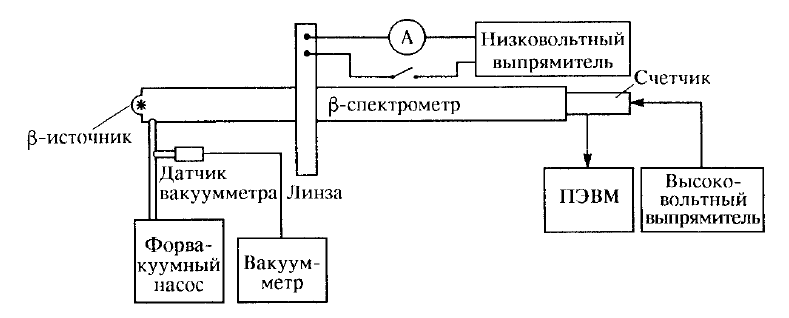
\includegraphics[width=\linewidth]{setup.png}
    \caption{Состав экспериментальной установки: 1 -- источник лазерного луча, 2 -- измеритель интенсивности (фотодиод), 3 -- микрометрический винт, 4 -- линза}
    \label{fig:setup}
\end{center}
\end{figure}

\section{Ход работы}

Измерим с помощью фотодиода, расположенного на подложке, перемещаемой микрометрическим винтом, распередение интенсивности лазерного пучка He-Ne-лазера в поперечном сечении. Построим график зависимости напряжения (интенсивности пучка) от поперечной координаты и аппроксимируем данный график гаусовой кривой, \linebreak полуширину  ($\sigma$) которой найдем из аппроксимации

\begin{figure}[h!]
    \centering
    \includegraphics[width = \linewidth]{graph1 (without lense).png}
    \caption{Зависимость напряжения на фотодиоде от его поперечной координаты \linebreak (без линзы, $\sigma_0 = 0,2 мм$, расстояние до фотокатода L = 60,5 см)}
    \label{fig1:without lense}
\end{figure}

\pagebreak

Поставим на пути лазерного пучка линзу, на расстоянии L = 35 см от источника лазерного пучка и снимем аналогичную зависимость

\pagebreak

\begin{figure}[h!]
    \centering
    \includegraphics[width = \linewidth]{graph2 (with lense).png}
    \caption{Зависимость напряжения на фотодиоде от его поперечной координаты \linebreak (с линзой, $\sigma_f = 1,28 мм$)}
    \label{fig2:wit lense}
\end{figure}

\subsection{Оценка фокусного расстояния линзы}

Пусть слева на линзу, расположенную в плоскости, перпендикулярно к ней падает гауссов световой пучок с плоским волновым фронтом. Тогда, пользуяюсь правилом ABCD:

$$
    q_2 = \frac{A q_1 + B}{C q_1 + D},
$$

где $A = 1 - l_2/f, \ B = l_1 + l_2 - l_1 l_2 / f, \  C = -1/f, \ D = 1 - l_1/f$

Приравнивая мнимые части данного равенства получаем:

$$
    \sigma^2_f = \sigma^2_0 \left(1 - \frac{l_1}{f} \right)^2 + \left( \frac{\lambda}{\pi \sigma_0 f} \right)^2 
$$

Решая данное уравнение относительно $f$ находим что $f \approx 63$ мм


\newpage

\section*{Приложение 1. Дополнительные задачи}

\subsection*{\S 1 № 1}

\begin{figure}[h!]
    \centering
    \includegraphics[scale = 0.4]{CQ1_1st.png}
    \includegraphics[scale = 0.4]{CQ1_2nd.png}
    \label{fig2:wit lense}
\end{figure}

\pagebreak


\subsection*{\S 1 № 2}

\begin{figure}[h!]
    \centering
    \includegraphics[scale = 0.4]{CQ2.png}
    \label{fig2:wit lense}
\end{figure}

\subsection*{\S 1 № 4}

\begin{figure}[h!]
    \centering
    \includegraphics[scale = 0.4]{CQ4.png}
    \label{fig2:wit lense}
\end{figure}

\pagebreak

\subsection*{\S 2 № 1}

Найти расходимость гауссова пучка нулевого порядка, у которого в плоскости z = 0 радиус фазового фронта $R_0$.

    

\begin{gather}
M = \begin{pmatrix}
       1 & z\\
        0 & 1
    \end{pmatrix} 
    \Rightarrow q_2 = q_1 + z\; ; \frac{1}{q_2} = \frac{1}{q_1 + z}\\
    q_1 = \frac{1}{\frac{1}{R_0} - i \frac{\lambda }{\pi \omega_0 ^2 }} = \frac{\frac{1}{R_0} + i \frac{\lambda }{\pi \omega_0 ^2}}{\left(\frac{1}{R_0}\right)^2 + \left(\frac{\lambda }{\pi \omega_0 ^2 }\right)^2} = A \left({\frac{1}{R_0} + i \frac{\lambda }{\pi \omega_0 ^2}}\right)\\
    \frac{1}{q_2} = \frac{1}{R\left(z\right) - i \frac{\lambda}{\pi \omega\left(z\right)^ 2}} = \frac{1}{A\left({\frac{1}{R_0} + i \frac{\lambda }{\pi \omega_0 ^2}}\right) + z}     = \frac{1}{\left(\frac{A}{R_0} + z\right)^ 2 + \left(\frac{\lambda}{\pi \omega_0 ^ 2} A\right) ^ 2}\\
    \Rightarrow \frac{ \lambda}{\pi \omega \left(z\right) ^ 2 } = \frac{\frac{\lambda }{\pi \omega_0 ^ 2} A}{ \left(\frac{A}{R_0} + z\right)^ 2 + \left(\frac{\lambda}{\pi \omega_0^ 2} A\right)^2}\\
    \omega\left(z\right)^2 = \frac{\left(\frac{A}{R_0} + z\right)^ 2 + \left(\frac{\lambda}{\pi \omega_0^ 2} A\right)^2}{ A \frac{1 }{\omega_0 ^ 2}}\\
    \theta_0 = \lim_{z \to \infty}\frac{\omega\left(z\right)}{z}
    = \sqrt{\lim_{z\to\infty}\frac{\omega\left(z\right) ^ 2}{z^2}} = \sqrt{\frac{A}{\omega_0^2}}  = \left[\omega_0 \sqrt{\left(\frac{1}{R_0}\right)^ 2  + \left(\frac{\lambda}{\pi \omega_0 ^ 2 }\right)^ 2}\right]^{-1}
\end{gather}
\textit{Ответ: }$\theta_0 = \left[\omega_0 \sqrt{\left(\frac{1}{R_0}\right)^ 2  + \left(\frac{\lambda}{\pi \omega_0 ^ 2 }\right)^ 2}\right]^{-1}$

\subsubsection*{№ 2}
Найти расходимость гауссова пучка n-го порядка, у которого в плоскости $z = 0$ фазовый фронт плоский.

Рассмотрим прохождение гауссова пучка нулевого порядка через свободное пространство. Положим, что в плоскости $z = 0$ фазовый фронт луча плоский, поэтому $1/q_1 = -i\lambda/{\pi\omega_0^2}$. Через вид лучевой матрицы свободного пространства имеем $q_2 = q_1 + z$ или $1/q_2 = 1/(q_1 + z)$. Учитывая формулу (\ref{equ:form}) и приравнивая почленно действительные и мнимые части выражения, получаем

\begin{equation}
    \omega_2^2(z) = \omega_0^2 (1 + (\frac{\lambda z}{\pi\omega_0^2})^2),
    \label{equ:zero1}
\end{equation}

\begin{equation}
    R_2(z) = z(1 + (\frac{\pi\omega_0^2}{\lambda z})^2).
    \label{equ:mage_of_chaos}
\end{equation}

Используя формулу (\ref{equ:zero1}), легко оценить угол расходимости $\theta_0$ в дальней зоне

\begin{equation}
    \theta_0 = \lim_{z\to\infty} \frac{\omega_2(z)}{z} = \frac{\lambda}{\pi\omega_0}.
\end{equation}



\subsubsection*{№ 3}
На линзу с фокусным расстоянием $f$ падает гауссов пучок с плоским фазовым фронтом и с поперечным размером $\omega_0$. Найти расстояние от линзы, на котором пучок будет иметь минимальный поперечный размер. Каков этот размер?



%\subsubsection{№ 4}
%На оптическую систему № 6 ($l_1 = 0,5\; м, l_2 = 1,0\; м, f = 0,5\; м$) под углом $\alpha = 0,01$ падает гауссов пучок нулевого порядка с $q = i (\lambda = 1\; мкм)$. Найти распределение поля на выходе системы.

%\subsection{\S 2}



%\textbf{1.} Найдите лучевую матрицу ГОС при смене направления прохождения системы на обратное.

%\begin{equation*}
%    \begin{pmatrix}
%        x_2\\
%        \alpha_2
% %    \end{pmatrix}
%     =
%     \textbf{M}
%     \begin{pmatrix}
%         x_1\\
%         \alpha_1
%     \end{pmatrix}
%     \Rightarrow
%     \begin{pmatrix}
%         x_1\\
%         \alpha_1
%     \end{pmatrix}
%     =
%     \textbf{M}^{-1}
%     \begin{pmatrix}
%         x_2\\
%         \alpha_2
%     \end{pmatrix}
% \end{equation*}
%
%\textit{Ответ:} $\textbf{M}_{обр} = \textbf{M}^{-1}$.

\pagebreak

\subsection*{Задачи}

\textbf{2.} 

\begin{figure}[h!]
    \centering
    \includegraphics[scale = 0.5]{Task1.png}
    \includegraphics[scale = 0.5]{Task2.png}
    \label{fig2:wit lense}
\end{figure}

\pagebreak

\begin{figure}[h!]
    \centering
    \includegraphics[scale = 0.5]{Task3.png}
    \includegraphics[scale = 0.5]{Task3_2nd.png}
    \label{fig2:wit lense}
\end{figure}

\pagebreak

%\textbf{3.} Стеклянная линза толщиной 30 мм вдоль оси имеет выпуклую входную поверхность с радиусом кривизны 50 мм и вогнутую выходную поверхность с радиусом кривизны 20 мм. Первая поверхность расположена слева и граничит с воздухом, вторая -- справа от неё и граничит с жидкостью, показатель преломления которой 1,4. Показатель преломления стекла 1,5. Найдите фокусные расстояния системы и укажите положения фокусов.

% TODO pic

\textbf{4.} Какой физический смысл в оптике лазерных пучков имеет матрица
$\begin{pmatrix}
       1 & 0\\
      -ip & 1
\end{pmatrix}$, где $p$ -- положительное действительное число?

Преобразуем эту матрицу, перенеся аргумент, связанный с $ip$ в знаменатель

\begin{equation*}%
\begin{pmatrix}
       1 & 0\\
       \frac{1}{i\frac{1}{p}} & 1
\end{pmatrix}
\end{equation*}

Поскольку из таблицы лучевых матриц известно, что матрица

\begin{equation*}
\begin{pmatrix}
       1 & 0\\
       -\frac{1}{f} & 1
\end{pmatrix}
\end{equation*}

соответствует линзе с фокусом f, то полученная нами матрица описывает линзу с мнимым фокусом $-\frac{1}{p}$, то есть рассеивающую линзу.

\textit{Ответ:} матрица описывает рассеивающую линзу с мнимым фокусом величиной $\frac{1}{p}$.

\textbf{5.} Изобразите поперечную структуру гауссовых пучков мод $U(x,y)_{m,n}$: TEM$_00$, TEM$_01$, TEM$_22$ (изображение на экране, перпендикулярном линии распространения луча).


\pagebreak

\begin{figure}[h!]
    \center{\includegraphics[width=4in]{patches.jpg}}
    \caption{Распределение интенсивности в сечении гауссова пучка для мод $m,n$ от 00 до 22. Слева-направо -- возрастание n, сверху-вниз -- рост m.}
    \label{fig:patches}
\end{figure}

\textbf{6.} Изобразите свободно распространяющийся вдоль оси Z гауссов пучок, если фазовый фронт в точке $z = 0$ плоский. Покажите линии фазового фронта в точках $z = 0, \pm L$.

\textbf{6.}Изобразите свободно распространяющийся гауссов пучок, вдоль оси Z, если фазовый фронт в точке z = 0 плоский.

См рисунок \ref{fig:zero_prop}

\textbf{7.} Выведите и постройте график зависимости радиуса волнового фронта гауссова пучка от расстояния.

Будем рассматривать прохождение гауссова пучка нулевого порядка через свободное пространство.

В плоскости z = 0 фронт плоский. Тогда можно считать, что $q_1 = -i \cdot \dfrac{\lambda}{\pi \omega_1^2}$

Для свободного пространства матрица ГОС имеет вид 
\begin{pmatrix}
1 & z\\
0 & 1
\end{pmatrix}.

Тогда, используя формулу ABCD \ref{equ:abcd} и выражение для q \ref{equ:form}, можно получить 

\begin{center}
    $R(z) = z + \dfrac{\omega_1^4 \pi^2}{\lambda^2 z}$
\end{center}

График этой зависимости имеет вид рис. \ref{fig:task8}:

\begin{figure}[H]
    \centering
    \includegraphics[width=10cm]{Task8.png}
    \caption{График зависимости R(z) - задание №7}
    \label{fig:task8}
\end{figure}

При z $\rightarrow$ $\inf$ $R(z) \sim z$, а при z $\rightarrow$ 0 $R(z) \sim \dfrac{1}{z}$. Кроме того, экстремум данной зависимости имеет место при $z = z_0 = \dfrac{\omega_1^2 \pi}{\lambda}$.

\textbf{8.} Дополните условие задачи 5 линзой (собирающей, рассеивающей), зеркалом (плоским, сферическим).

Рассмотрим преобразование по формуле ABCD \ref{equ:abcd}. Оно определит картину на экране при прохождении через линзу или отражении от зеркала.

Матрицы ГОС для линзы и сферического зеркала очень схожи: 

\begin{itemize}
    \item 
\begin{pmatrix}
1 & 0\\
-\dfrac{1}{f} & 1
\end{pmatrix} - линза
    \item 
\begin{pmatrix}
1 & 0\\
-\dfrac{2}{R} & 1
\end{pmatrix} - сферическое зеркало
\end{itemize}

При помощи \ref{equ:abcd} проведеём преобразования и получим:

\begin{center}
    $R_2 = \dfrac{R_1 f}{f - R_1}$ \hspace{2cm} $\omega_2 = \omega_1$
\end{center}

Как видим, будут только изменения в радиусе фронта волны, но поперечные размеры остаются прежними. Таким образом картина качественно не изменяется, потому что мы наблюдаем интенсивность, то есть квадрат модуля поля, а модуль комплексной части (в которой происходят все изменения) равен 1.

Для плоского зеркала считаем R $\rightarrow$ $\inf$. Тогда матрица будет единичной и никаких изменений в картине также не будет.

\textbf{9.} Изобразите изменение вдоль оси поперечного размера основной моды резонатора, образованного зеркалами (двумя плоскими, плоским и сферическим, двумя сферическими) и содержащего внутрирезонаторную линзу. Покажите линии фазового фронта.

\begin{figure}[htbp]
    \centering
    \includegraphics[width=10cm]{Task9/Page1.png}
    \includegraphics[width=10cm]{Task9/Page2.png}
    \label{fig:task9_1}
\end{figure}

\begin{figure}[htbp]
    \centering
    \includegraphics[width=10cm]{Task9/Page3.png}
    \includegraphics[width=10cm]{Task9/Page4.png}
    \label{fig:task9_2}
\end{figure}

\begin{figure}[htbp]
    \centering
    \includegraphics[width=10cm]{Task9/Page5.png}
    \label{fig:task9_3}
\end{figure}

\textbf{10.} В He-Ne лазере ($\lambda = 0,6328\; мкм$) используется конфокальный (фокусы зеркал совпадают) резонатор длиной $L = 1\; м$. Вычислите размер пятна в центре резонатора и на зеркалах.
\begin{center}
\begin{minipage}[t]{0.15\linewidth}
    \textbf{Дано:}
    
  $\lambda = 632.8 \; нм$
  
  $L = 1 \; м $
   
    \vspace{0.1in}
    \hrule
    \vspace{0.1in}
    $\omega_з - ?$
    
    $\omega_р - ? $
\end{minipage}
\vline
\begin{minipage}[t]{0.65\linewidth}
\setlength{\parindent}{2ex}
    \textbf{Решение:}
    
    В центре резонатора:
    \begin{equation*}
        \omega_р = \sqrt{\frac{L \lambda }{2 \pi}} = 0.317 \; нм
    \end{equation*}
    
    На зеркалах:
    \begin{equation*}
        \omega_з = \sqrt{L \lambda }{\pi} = 0.449 \; нм
    \end{equation*}
\end{minipage}
\end{center}
\textit{Ответ:}$\; \omega_р = 0.317 \; нм ; \; \omega_з =0.449 \; нм$

%\subsubsection{КВ № 11}
%\textbf{11.} В CO$_2$ лазере ($\lambda = 10,6\; мкм$) используется полуконфокальный (фокус сферического зеркала совпадает с расположением плоского зеркала) резонатор длиной $L = 2\; м$. Вычислите размер пятна в центре резонатора и на зеркалах.

\textbf{12.} Смесь гауссовых пучков до $n$-го порядка включительно с характерным поперечным размером $\sigma_1$ падает на оптическую систему № 6, $l_1 = l_2 = f$. На выходе системы поперечный размер пучка равен $\sigma_2$. Исходя из величины $\sigma_1$ и $\sigma_2$, определить $n$ и значение параметра $\omega_0$ на входе системы. Рассмотреть случай плоского и не плоского фрона пучка на входе в систему.

Решение : 

Для оптической системы 6 при $l_1 = l_2 = f  $ лучевая матрица имаеет вид
\[
\begin{pmatrix}
       0 & f\\
       - \frac{1}{f} & 0
\end{pmatrix}
\]
Тогда по закону ABCD:

\begin{gather*}
     q_2 = \frac{A q_1 + B}{C q_1 + D} = \frac{0 \cdot q_1 + f}{ -\frac{1}{f} q_1 + 0} = - f^ 2 \frac{1}{q_1}\\
     \frac{1}{q} = \frac{1}{R} - i\frac{\lambda}{\pi \omega^ 2} \Rightarrow 1/ \left(\frac{1}{R_2} - i \frac{\lambda}{\pi \omega_2^2} \right)  = - f^2 \left( \frac{1}{R_1} - i \frac{\lambda}{\pi\omega_1 ^ 2} \right)\\
    \left(\frac{1}{R_2}  + i \frac{\lambda}{\pi \omega_2^2} \right)/ \left( \left(\frac{1}{R_2}\right) ^ 2 + \left( \frac{\lambda}{\pi \omega_2^2}\right)^ 2  \right) = - f^2 \left( \frac{1}{R_1} - i \frac{\lambda}{\pi\omega_1 ^ 2} \right)
\end{gather*}

Рассмотрим случай плоского фронта волны : $1/R = 0$. Тогда выражение примет вид:
\begin{equation*}
     \left(\frac{1}{R_2}  + i \frac{\lambda}{\pi \omega_2^2} \right)/ \left( \left(\frac{1}{R_2}\right) ^ 2 + \left( \frac{\lambda}{\pi \omega_2^2}\right)^ 2  \right) =  i f^2\frac{\lambda}{\pi\omega_1 ^ 2} 
\end{equation*}
Приравнивая действительную и мнимую части выражения получем, что $1/R_2 = 0 $ и , следовательно, 
\begin{equation*}
    \frac{\pi \omega_2^2} {\lambda }  = f^2 \frac{\lambda }{\pi \omega_1 ^ 2} 
\end{equation*}
Отсюда $\omega_2 = f\lambda / \pi \omega_1 $и 
\begin{gather*}
     \frac{\omega_2}{\omega_1} = \frac{\sigma_2}{\sigma_1} = \frac{f \lambda}{\pi\omega_1^2}\\
     \omega_1^2 = \frac{f \lambda}{\pi}\frac{\sigma_1}{\sigma_2} = \frac{\sigma_1 ^ 2}{2m + 1}\\
     m = \left(\sigma_1\sigma_2\frac{\pi}{f \lambda} - 1\right) / 2
\end{gather*}
   
\textit{Ответ:} $\omega_1 = \sqrt{\frac{f \lambda}{\pi}\frac{\sigma_1}{\sigma_2}} \; ; \; m = \left(\sigma_1\sigma_2\frac{\pi}{f \lambda} - 1\right) / 2 $




%\subsubsection{КВ № 13}
%\textbf{13.} Проведите рассчёт характеристик резонатора длиной $2l$, образованного сферическим (радиуса $R$) и плоским зеркалом, с внутрирезонаторной апертурой ширины $D$, расположенной в центре резонатора.% Расчёт проводить для конкретных значений параметров $R, l, D$.

%\subsubsection{КВ № 14}
%\textbf{14.} Смесь гауссовых пучков до $n$-го порядка включительно с заданным значением параметра $\omega$ и $1/R_0 \ne 0$ падает на линзу с фокусным расстоянием $f$. Найти минимальный размер пучка за линзой и расстояние от линзы до перетяжки.

%\subsubsection{КВ № 15}
%\textbf{15.} Найти собственную моду бесконечной системы периодически расположенных одинаковых линз с фокусным расстоянием $f$ и расстоянием между 



\end{document}
